\chapter{Reliable SoTS Through Orthogonal State Modeling}
\label{ch:reliable-sots}

Systems of Twinned Systems (SoTS) combine System-of-Systems (SoS) composition with Digital Twin-enabled reflection and coordination. While this integration enables adaptive, data-driven decision-making across autonomous constituents, it also increases sensitivity to structural and operational disturbances. Participation changes and performance impairments may propagate across both physical and digital layers, affecting mission fulfilment.

The systematic literature review presented in Chapter~\ref{ch:literature-review} shows that reliability is widely acknowledged in SoTS research but is rarely formalized as an architectural modeling dimension. In parallel, participation and lifecycle models govern structural belonging without explicitly conditioning admissibility on operational state.

This chapter addresses this gap by introducing an orthogonal state modeling framework in which structural belonging and operational health are represented as interacting dimensions. Reliability is reframed as an architectural constraint over participation, enabling progressively stronger governance of admissible system configurations.

Throughout this chapter, key concepts are illustrated using a distributed microgrid SoTS example.
\begin{runningexample}{Running Example: CEP in a Microgrid SoTS}
Throughout this thesis, we consider a running example of a distributed microgrid composed of independently owned energy units that dynamically participate in grid-balancing operations, collectively forming a SoTS \cite{wullink2024foundational, monsalve2021novel, jiang2022novel}.

\begin{center}
\begin{tikzpicture}[
    font=\small,
    twin/.style={
        rectangle, draw, rounded corners,
        minimum width=2.4cm,
        minimum height=1cm,
        inner ysep=3pt,
        fill=white,
        align=center
    },
    dependency/.style={gray!60, thin},
    cep/.style={
        rectangle,
        draw,
        thick,
        fill=white,
        minimum width=4.5cm,
        align=center
    }
]

% SoS Boundary
\node[
    draw=black!60,
    thick,
    fill=white,
    rounded corners,
    minimum width=10.2cm,
    minimum height=4.4cm,
    label=above:{\textbf{SoTS}}
] (sos) at (0,0) {};

% Participating DTs
\node[twin] (dt1) at (-3,0.9)  {DT$_1$};
\node[twin] (dt2) at (0,1.2)   {DT$_2$};
\node[twin] (dt3) at (3,0.9)   {DT$_3$};
\node[twin] (dt4) at (-1.5,-1.1) {DT$_4$};
\node[twin] (dt5) at (1.5,-1.1)  {DT$_5$};

% Interdependencies
\draw[dependency] (dt2) -- (dt3);
\draw[dependency] (dt3) -- (dt5);
\draw[dependency] (dt4) -- (dt1);

% CEP
\node[cep, below=-0.15cm of sos.south]
{Complex Event Processing (CEP) Layer};

\end{tikzpicture}
\end{center}

Grid stability requires real-time balance between generation and demand while preserving voltage and frequency within safe bounds. DTs and CEP have been combined for distributed monitoring and coordination \cite{marah2025agent}. The SoTS includes a CEP layer that correlates Digital Twin event streams representing contribution, capacity, and grid conditions. This enables the system to detect instability and identify coordination and optimization opportunities.
\end{runningexample}



\section{Disturbances and SoS-Level Reliability}

In dependability theory, reliability is defined as the ability of a system to deliver correct and continuous service over time \cite{avizienis2001fundamental}. SoS, however, differ fundamentally from traditional systems due to the operational and managerial independence of their constituents \cite{maier1998architecting}. Constituents may join, leave, degrade, or evolve autonomously. Reliability in SoS  cannot be reduced to component-level correctness; it must be understood in terms of sustained mission fulfilment despite constituent autonomy and variability.

\citet{ferreira2023towards} define a disturbance in SoS as any structural or operational change that alters the availability or effective execution of capabilities required for mission fulfilment. Disturbances may arise from participation changes, performance degradation, coordination misalignment, or other variations in constituent behavior. Following \cite{ferreira2023towards}, reliability in SoS is therefore characterized as the ability of the system to tolerate such disturbances while continuing to fulfil its mission objectives.


\section{Why SoTS Requires Architectural Reliability}

In traditional SoS, a degraded constituent may reduce local performance without necessarily destabilizing the entire system. In SoTS, however, digital twin coupling fundamentally alters this dynamic.

Operational state is continuously exposed, aggregated, and used to inform coordination decisions. System-level behavior may depend on distributed state estimation and event correlation. An impaired constituent therefore does not merely underperform locally; it may distort shared system knowledge, misinform adaptation logic, and propagate instability through coordination mechanisms.

If structurally active but operationally impaired constituents remain admissible, several systemic risks arise:
\begin{itemize}
    \item Aggregated state estimation may become inaccurate,
    \item CEP-based coordination may trigger incorrect control actions,
    \item Disturbances may cascade across interdependent constituents.
\end{itemize}

\begin{runningexample}{Recall: Disturbances in the Microgrid SoTS}

In the microgrid SoTS, these risks manifest concretely. A Digital Twin leaving during peak demand may create an unexpected generation shortfall. A weakened unit that continues supplying unstable power may introduce frequency fluctuations across the grid. Delayed or corrupted measurements may prevent timely detection of imbalance, leading to inappropriate corrective actions.

\begin{center}
\begin{tikzpicture}[
    font=\footnotesize,
    twin/.style={
        rectangle, draw, rounded corners,
        minimum width=2.25cm,
        minimum height=0.9cm,
        inner ysep=2.5pt,
        fill=white,
        align=center
    },
    affected/.style={
        rectangle, draw=red, thick, rounded corners,
        minimum width=2.25cm,
        minimum height=0.9cm,
        inner ysep=2.5pt,
        fill=white,
        align=center
    },
    failed/.style={
        rectangle, draw=red, fill=red!20, thick,
        rounded corners,
        minimum width=2.25cm,
        minimum height=0.9cm,
        inner ysep=2.5pt,
        align=center
    },
    partially/.style={
        rectangle, draw=red, thick,
        rounded corners,
        minimum width=2.25cm,
        minimum height=0.9cm,
        inner ysep=2.5pt,
        fill=white,
        align=center
    },
    faded/.style={opacity=0.35},
    dependency/.style={gray!60, thin},
    disturbance/.style={red, very thick},
    disturbance_partial/.style={red, dashed, very thick},
    cep/.style={
        rectangle,
        draw,
        thick,
        fill=white,
        minimum width=4.35cm,
        align=center
    }
]

% DT1 after leaving
\node[twin] (dt1_out) at (-4.6,3.0) {DT$_1$};

% SoTS Boundary
\node[
    draw=black!60,
    thick,
    fill=white,
    rounded corners,
    minimum width=9.8cm,
    minimum height=4.1cm,
    label=above:{\textbf{SoTS}}
] (sos) at (0,0) {};

% Participating DTs
\node[twin,faded] (dt1) at (-2.9,0.85) {DT$_1$};

\node[failed]   (dt2) at (0,1.1)  {DT$_2$};
\node[affected] (dt3) at (2.9,0.85)  {DT$_3$};

\node[partially] (dt4) at (-1.45,-1.0) {DT$_4$};
\node[partially] (dt5) at (1.45,-1.0)  {DT$_5$};

% Interdependencies
\draw[dependency] (dt2) -- (dt3);
\draw[dependency] (dt3) -- (dt5);

% weakened dependency
\draw[gray!80, thin, dashed, ->] (dt1) -- (dt4);

% Disturbance propagation
\draw[disturbance, ->] (dt2) -- (dt3);
\draw[disturbance, ->] (dt3) -- (dt5);

% Leave transition
\draw[->, thick]
(dt1) to[out=115,in=-95]
node[left, font=\scriptsize, black!90]{left}
(dt1_out);

% CEP Layer
\node[cep, below=-0.12cm of sos.south] (cep)
{Complex Event Processing (CEP) Layer};

\end{tikzpicture}

\vspace{-4pt}
{\footnotesize Disturbance propagation within a SoTS:
\textcolor{red}{\(\rightarrow\)} propagation,
\tikz{\draw[red, thick, fill=red!20] (0,0) rectangle (0.25,0.25);} faulty DT,
\tikz{\draw[red, thick] (0,0) rectangle (0.25,0.25);} affected DT}
\end{center}

Because energy units are dynamically coordinated through shared state information, such disturbances do not remain local. Structural participation changes, operational degradation, or incorrect state propagation directly influence system-level stability and mission fulfilment.

\end{runningexample}

These observations illustrate a critical distinction: in SoTS, participation without operational regulation can amplify disturbance rather than contain it. Reliability must therefore operate as an architectural constraint over participation, ensuring that structurally active constituents are also operationally admissible.





\section{Disturbances Along Two Primary Dimensions}
Reliability in a SoTS is tied to sustained mission fulfilment despite disturbances. Mission fulfilment depends on the presence and effective execution of constituent capabilities. Disturbances arise when constituents are either absent/leave or operationally degraded.

Two primary and orthogonal dimensions define these alterations: belonging and health.
\begin{center}
\footnotesize
\begin{tabular}{p{2.5cm}|p{6cm}|p{6cm}}
& \textbf{Healthy} & \textbf{Unhealthy} \\
\hline
\textbf{Belongs}
& \textbf{Stable participation.} 
\newline Capabilities are available and effectively delivered, supporting mission fulfilment without introducing disturbance.
& \textbf{Degraded participation.} 
\newline Capabilities are available but delivered below expected performance, introducing operational disturbances that may influence dependent constituents. \\

\textbf{Does not belong}
& \textbf{Structural withdrawal.} 
\newline Operationally capable but structurally absent; its departure may disrupt dependent constituents and alter mission performance.
& \textbf{Externalized disturbance.} 
\newline Structurally absent and operationally impaired; instability originates outside the SoTS but may affect it upon re-entry. \\
\end{tabular}
\end{center}



\paragraph{Dimension 1 — Belonging.}

Participation in SoS is voluntary and autonomous \cite{salado2015abandonment}. Constituents may abandon the SoS or withhold participation, dynamically altering the architectural composition. Salado et al. observe that such abandonment has systemic consequences, as removal of a constituent reduces the collective capability available to achieve mission objectives.

Belonging therefore captures structural participation:

\begin{itemize}
    \item \emph{Belongs} — structurally present and contributing capabilities.
    \item \emph{Does not belong} — structurally absent and unable to contribute.
\end{itemize}


\paragraph{Dimension 2 - Health.}
Even when present, a constituent may fail to meet its objectives due to faults or internal degradation. \cite{ferreira2023towards} emphasize that faults reduce a constituent's ability to achieve its intended performance, thereby diminishing its effective capability contribution.

Health therefore captures the operational quality of capability provision:

\begin{itemize}
    \item \emph{Healthy} - capabilities are delivered in alignment with expected objectives.
    \item \emph{Unhealthy} - capability delivery is degraded or impaired.
\end{itemize}



Belonging determines whether capability is available within the SoTS. Health determines whether capability is effectively delivered. These dimensions are analytically independent but operationally interacting.


Disturbances in SoTS emerge from structural changes in participation, faults or impaired performance within constituents, or both. Because both mechanisms affect the presence or effective execution of capabilities, ensuring reliability in SoTS requires architectural regulation of participation across these dimensions.



\section{Proposal: Evaluating Reliable SoTS through Orthogonal State Modelling} - Condense this down a lot and combine with the next section
Research on SoS has modeled the different states a constituent may occupy during operation \cite{axelsson2019refined, svenson2020situation, hristozov2023modeling, dridi2022maude, baumgart2021model}. These participation models define how constituents join, remain in, or leave the SoS, specifying the conditions under which they are permitted to contribute to overall system-level capability.

In parallel, reliability research defines SoS reliability as the ability to sustain system performance under disturbance \cite{ferreira2023towards, li2025reliability}. At the SoS level, reliability concerns detecting faults, tolerating disturbances, reconfiguring when necessary, and preserving overall capability \cite{ferreira2024framework, uday2015designing, garro2014reliability}.

Although both lines of research are concerned with the capability delivered by the SoS, they are developed independently. Participation decisions are typically based solely on lifecycle conditions, without explicit consideration of a constituent's operational state. Consequently, problems within constituents are addressed after they affect performance, rather than influencing participation decisions in advance.

There is therefore no explicit architectural mechanism that links operational condition to participation. A constituent may remain part of the SoS as long as lifecycle criteria are satisfied, even when its current operational state threatens overall mission stability. Given that reliability is widely acknowledged yet rarely formalized at the architectural level, and given that participation models do not condition contribution on operational state, a modeling framework that explicitly integrates these dimensions is required.


\subsection{Orthogonal Modeling of Belonging and Health}

I propose an orthogonal lifecycle modeling framework in which belonging and health are represented as parallel state regions. Each constituent occupies a configuration in the belonging–health disturbance space introduced earlier. 

Transitions in the participation dimension are guarded by conditions in the health dimension. Structural transitions (e.g., join, remain, leave) are therefore not solely governed by autonomy or mission demand, but may be constrained by operational state.

Orthogonality ensures that structural and operational evolution remain analytically distinct while permitting controlled interaction. Belonging captures structural participation; health captures operational condition. Their interaction determines the admissible configurations of a constituent within the SoTS.



\section{Proposed Orthogonal Lifecycle Reliability Framework}

To integrate structural participation and operational condition, I propose an orthogonal lifecycle reliability framework in which participation is governed by two formally distinct but interacting state dimensions.

Let
\[
B
\]
denote the set of belonging states, and
\[
H
\]
denote the set of health states.

The composite participation state of a constituent is defined as the Cartesian product:
\[
S = B \times H
\]

Each composite state \( s = (b,h) \in S \) represents a structural--operational configuration.

Reliability is defined as an architectural admissibility constraint over \(S\). For a reliability level \(R\), let:
\[
S_R \subseteq S
\]
denote the subset of participation configurations permitted under that level. Higher reliability levels impose progressively stricter admissibility constraints:
\[
S_{R+1} \subseteq S_R
\]

Transitions in the belonging dimension are conditioned on health predicates:
\[
\delta_B : B \times H \rightarrow B
\]
such that structural participation is regulated by operational state.

This formulation elevates reliability from reactive disturbance handling to proactive participation governance.





\subsection{Instantiation in State Charts}
I now demonstrate the proposed modellling grounded in the running example explored above, using state charts \cite{}

The formalization below is grounded in the motivating SoTS use case \ref{use-case} presented earlier. While the specific states reflect that scenario, the orthogonal modeling structure is domain-agnostic and can be instantiated with alternative belonging, health, and admissibility definitions as required.



\section{Instantiation of the Belonging Dimension}

The belonging dimension is grounded in the lifecycle model proposed by Axelsson et al.~\cite{axelsson2019refined}:

\[
B =
\{\textit{Disengaged}, \textit{Prepared}, \textit{Passive}, \textit{Active}\}
\]

These states capture structural integration within the SoTS.


Grounded in the constituent lifecycle model proposed by \cite{axelsson2019refined}, the initial set of belonging states is defined as:
\begin{equation*}
B = \{ \textit{Disengaged}, \textit{Prepared}, \textit{Passive}, \textit{Active} \}
\end{equation*}

\begin{itemize}\setlength{\itemsep}{0pt}\setlength{\parskip}{0pt}
    \item \textit{Disengaged} (renamed from \textit{Ignorant}): the constituent does not structurally participate in the SoTS.
    \item \textit{Prepared}: the constituent is capable of participation but not yet structurally engaged.
    \item \textit{Passive}: the constituent participates with limited coordination or influence.
    \item \textit{Active}: the constituent is fully integrated and actively coordinated within the SoTS.
\end{itemize}


\section{Instantiation of the Health Dimension}

The health dimension is grounded in classical dependability theory \cite{avizienis2004basic, parhami1994multi}. We define:

\[
H =
\{
\textit{Ideal},
\textit{Defective},
\textit{Faulty},
\textit{Erroneous},
\textit{Malfunctioning},
\textit{Degraded},
\textit{Failed}
\}
\]

These states reflect increasing deviation from intended capability delivery.


Grounded in \cite{parhami1994multi} multi-level reliability model, system impairment is characterized through seven operational states representing progressive degradation:
\begin{equation*}
H = \{ \textit{Ideal}, \textit{Defective}, \textit{Faulty}, \textit{Erroneous}, \textit{Malfunctioning}, \textit{Degraded}, \textit{Failed} \}
\end{equation*}

\begin{itemize}\setlength{\itemsep}{0pt}\setlength{\parskip}{0pt}
    \item \textit{Ideal}: no defects or impairments are present.
    \item \textit{Defective}: latent defects exist but have not yet activated.
    \item \textit{Faulty}: active faults are present internally.
    \item \textit{Erroneous}: internal state corruption has occurred.
    \item \textit{Malfunctioning}: incorrect behavior is externally observable.
    \item \textit{Degraded}: service is delivered with reduced capability.
    \item \textit{Failed}: required service can no longer be delivered.
\end{itemize}




\section{Fault Tolerance as Architectural Response}

Let
\[
\Phi : S \rightarrow P
\]
denote a mapping from composite participation states to a set of fault tolerance patterns \(P\) \cite{hanmer2013patterns}.

This mapping associates disturbance configurations with architectural responses. Fault tolerance thus becomes structurally embedded within participation governance rather than applied solely after failure.




\section{Reliability Levels}

I now present the state charts corresponding to each reliability level. Each level extends the previous one by progressively strengthening architectural control over participation and constraining the admissible combinations of lifecycle belonging and operational health.

\subsubsection{Level 1 - Reactive}
\begin{figure}[htp]
\centering
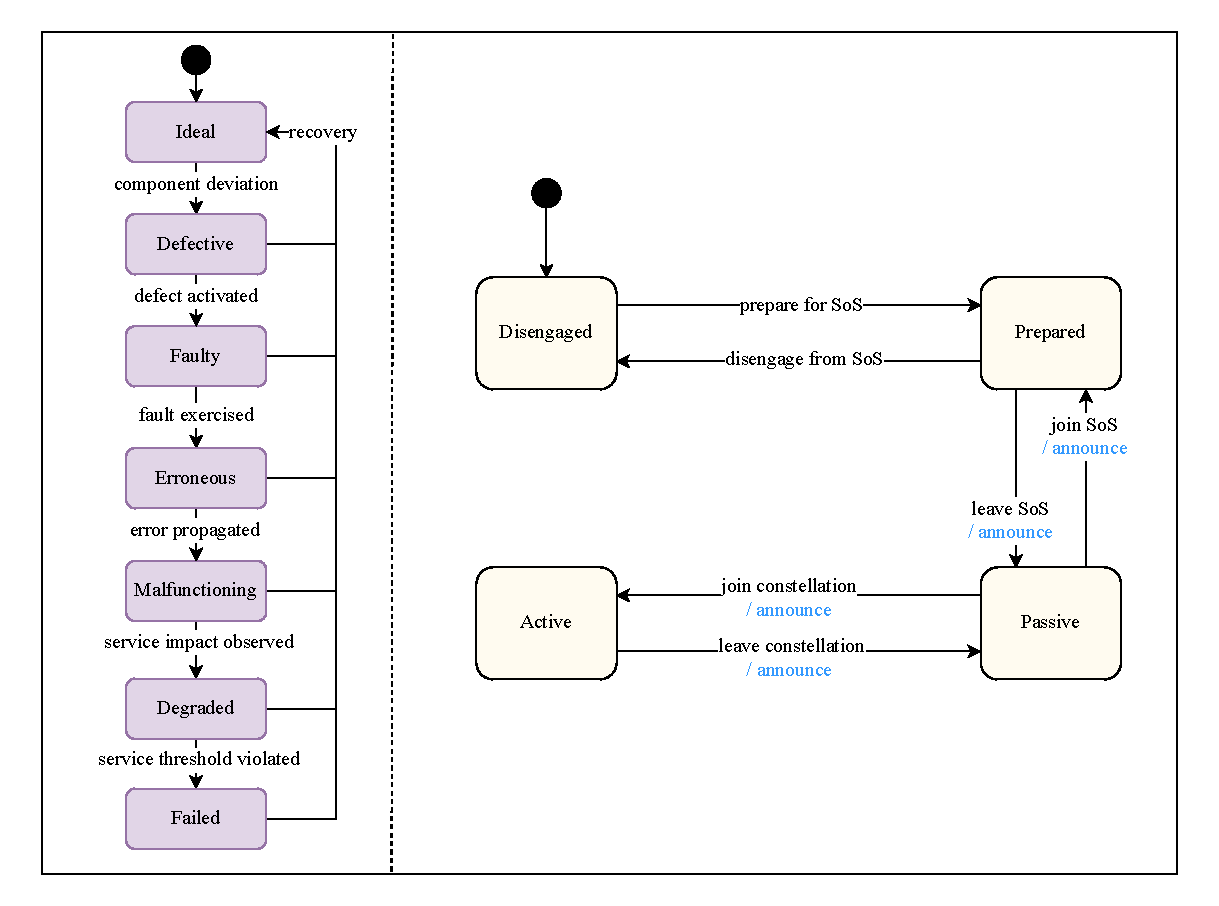
\includegraphics[width=0.8\linewidth]{figures/Approach/lv1.pdf}
\caption{Level 1: Reactive}
\label{fig:lv1}
\end{figure}

Level 1 reflects the most loosely coupled and least regulated form of SoTS. Following \cite{axelsson2019refined}, constituents are required to make participation changes visible to the SoS. We instantiate this architecturally by enforcing mandatory \textit{announcement} actions on all lifecycle transitions, including joining or leaving the SoS and joining or leaving a constellation, as shown in Figure~\ref{fig:lv1}. At this level, the two regions evolve independently. No architectural guards regulate admissible combinations of health and belonging.

This represents the weakest form of architectural control. Participation is made observable through mandatory announcements, but operational health does not regulate admission or continued involvement.

Such a configuration aligns naturally with highly collaborative or virtual SoTS, where constituents retain autonomy and central governance is minimal. The SoTS therefore operates reactively, responding to disturbances only after they become externally visible.


\subsubsection{Level 2 - Proactive}
\begin{figure}[htp]
\centering
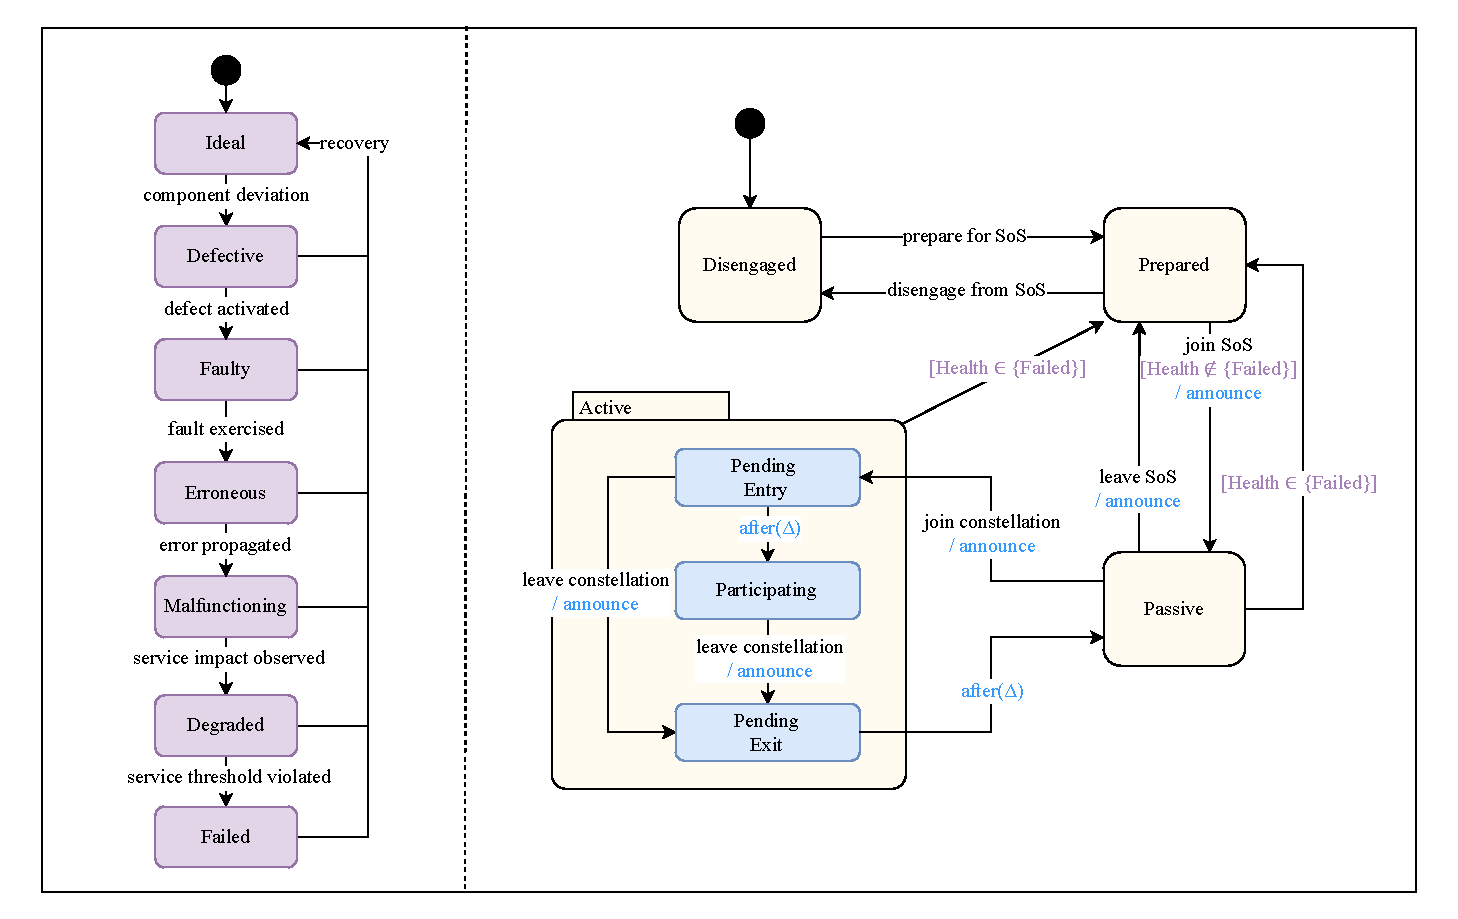
\includegraphics[width=0.9\linewidth]{figures/Approach/lv2.pdf}
\caption{Level 2: Proactive}
\label{fig:lv2}
\end{figure}

Level 2 introduces reliability-aware governance by coupling operational health to participation. Mandatory \textit{announcement} actions remain enforced on all lifecycle transitions, but health now constrains admissible combinations of belonging and activity, as shown in Figure~\ref{fig:lv2} 

If $Health \in {Failed}$ while in the \textit{Active} or \textit{Passive} state, the architecture initiates an exit sequence. This ensures that failed constituents cannot remain actively participating in a constellation. Admission is also guarded: the transition \textit{join SoS} is permitted only when $Health \notin {Failed}$, preventing failed constituents from entering the system.

The \textit{Active} state is refined into three substates: \textit{Pending Entry}, \textit{Participating}, and \textit{Pending Exit}. Temporal delays (e.g., \textit{after($\Delta$)}) are present during transitions from \textit{Pending Entry → Participating} and from \textit{ Pending Exit → Passive}. These delays assist with disturbance handling. During entry, the delay allows a constituent to stabilize before fully participating. During exit, the delay ensures withdrawal is controlled rather than abrupt, reducing the risk of sudden disruption to other participants. 

This level aligns most naturally with \textit{Directed} and \textit{Acknowledged SoTS}, where centralized oversight exists and basic containment of disturbances is required, and is less typical of highly autonomous \textit{Collaborative} or \textit{Virtual SoTS}.


\subsubsection{Level 3 - Controlled}
\begin{figure}[htp]
\centering
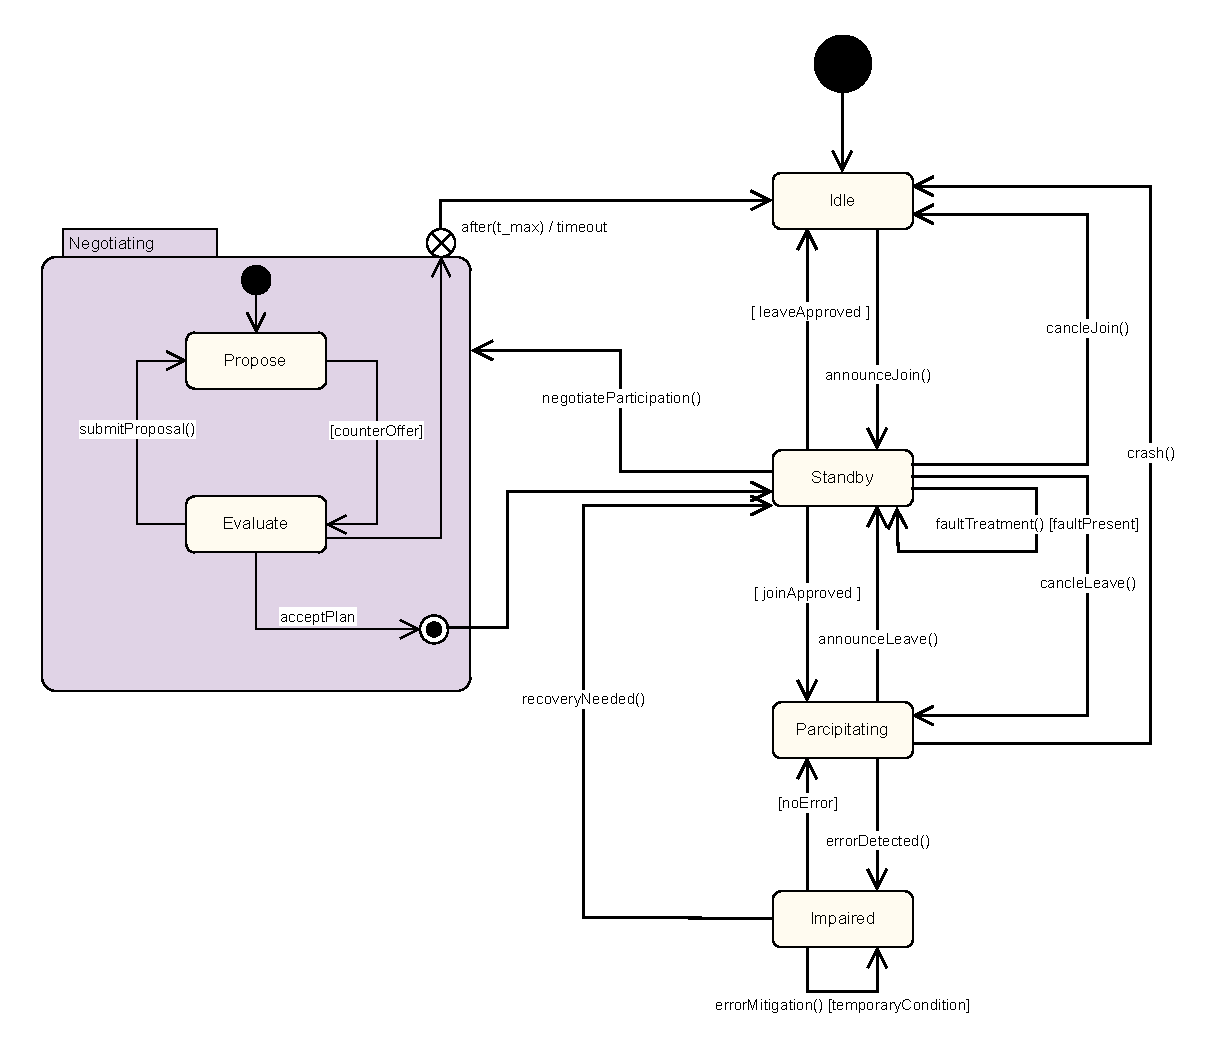
\includegraphics[width=\linewidth]{figures/Approach/lv3.pdf}
\caption{Level 3: Controlled}
\label{fig:lv3}
\end{figure}

Level 3 strengthens architectural regulation by introducing explicit negotiation and tighter participation control. Mandatory \textit{announcement} actions remain enforced, and this level includes all health-based constraints and stabilization mechanisms introduced in Level 2.

Admission to a constellation is now mediated through a negotiation phase within the \textit{Passive} state, which is refined into \textit{Available} and \textit{Negotiating}. A constituent may transition into negotiation depending on its health condition. If issuing a \textit{join request}, the constituent must be in ideal health ($Health \in {Ideal}$). If receiving a \textit{join invitation}, a constituent may be admitted in an operational but not perfect state ($Health \in {Ideal, Defective, Faulty}$), reflecting scenarios where the SoTS may require additional capacity despite minor impairments.

Active participation remains structured through \textit{Pending Entry}, \textit{Participating}, and \textit{Pending Exit}. However, exit is no longer voluntary. A constituent must issue a \textit{leave request}, and departure may be denied (\textit{exitDenied}) if architectural conditions are not satisfied. This prevents destabilizing during critical phases.

Unlike Level 2, participation is no longer only health-constrained. It is also regulated through negotiation and controlled admission and exit decisions. Lifecycle evolution becomes an explicitly governed process. This level aligns most naturally with \textit{Directed SoTS} and strongly governed \textit{Acknowledged SoTS}, where coordinated control and regulated participation are required.



\subsubsection{Level 4 - Adaptive}
\begin{figure}[htp]
\centering
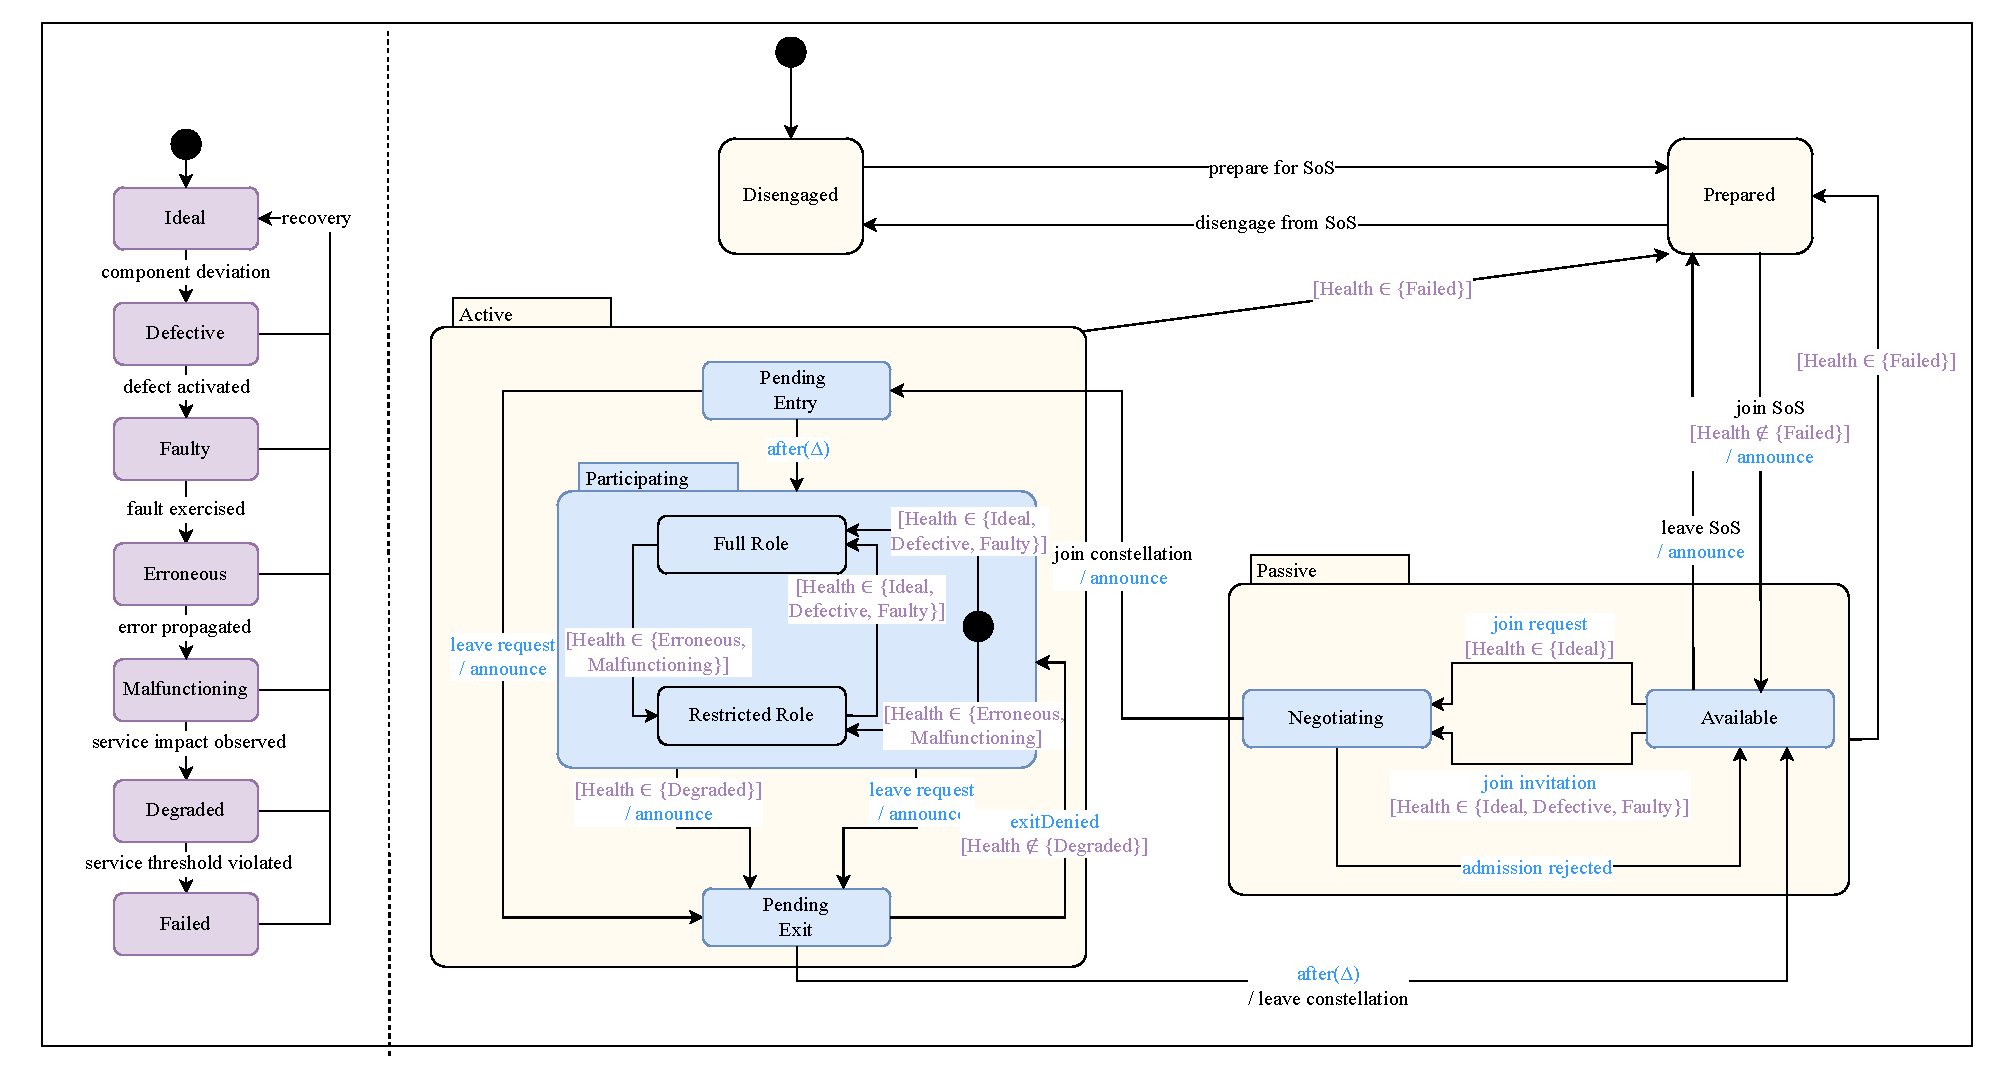
\includegraphics[width=\linewidth]{figures/Approach/lv4.pdf}
\caption{Level 4: Adaptive}
\label{fig:lv4}
\end{figure}

Level 4 extends Level 3 by introducing role adaptation based on operational health. All enforcement mechanisms from the previous levels remain in place: mandatory announcements, guarded admission, negotiated entry, controlled exit, stabilization delays, and failure-triggered disengagement.

The key refinement occurs within the \textit{Participating} state. The state is decomposed into two roles: \textit{Full Role} and \textit{Restricted Role}. Health now determines not only whether a constituent may participate, but how it participates.

When $Health \in {Ideal, Defective, Faulty}$, the constituent may operate in a \textit{Full Role}. If health degrades to $Health \in {Erroneous, Malfunctioning}$, participation is downgraded to a \textit{Restricted Role}. In this mode, the constituent remains part of the constellation but operates with reduced responsibility, limiting the potential propagation of disturbance.

Level 4 no longer waits for complete failure to enforce exit. When $Health \in {Degraded}$, the architecture proactively initiates a leave request, triggering a controlled withdrawal with proper notice. Failure still results in enforced disengagement, but intervention now occurs earlier to limit disturbance propagation.

Level 4 enables adaptive containment: degraded constituents can be functionally reconfigured before removal. Disturbance handling therefore shifts from reactive containment (Level 2) and negotiated control (Level 3) to dynamic role reconfiguration.

This level aligns most naturally with strongly governed \textit{Directed SoTS}, and advanced \textit{Acknowledged SoTS}, where architectural intelligence, often embodied in a coordinating Digital Twin, can assess health and reassign responsibilities in real time.



